% Copyright (c) 2008-2009 solvethis
% Copyright (c) 2010-2016,2018-2019,2021 Casper Ti. Vector
% Copyright (c) 2021 Kurapica
% Copyright (c) 2021 iofu728
% Overleaf version.

%*********************************************************************
% iofu728-pkuthss: 北京大学研究生学位论文模板
% 2021/06/09 v1.0.0
%
% 重要提示:
%   1. 当前overleaf版符合2021研究生学位论文要求,可通过图书馆审核
%   2. 当前版本基于pkuthss v1.9.0
%   3. 请使用UTF-8编码,XeLaTeX方式编译
%   4. 请仔细阅读用户文档
%   5. 修改、使用、发布本文档类请务必遵循LaTeX Project Public License和知识共享4.0
%   6. 如有疑问github/iofu728/pkuthss上提问或联系作者@iofu728
%*********************************************************************

\documentclass[fontset=fandol,ugly]{pkuthss}
  % 学位论文模式  ugly    (默认打开,请保留)
  % 盲审模式      blind   (默认关闭)
  % 字体库        fontset
  %   auto | windows | windows@overleaf | mac | fandol | ubuntu | none
  % windows*, mac为商业字体,如需使用请遵循相应版权协议(默认下overleaf中不可用)
  % fandol与windows效果相近,但字符库偏少,推荐使用(默认);
  % ubuntu字体效果偏差较大; 设为none时需自行配置字体集;

\usepackage[backend=biber,style=gb7714-2015]{biblatex}
  % 参考文献遵循GB/T 7714-2015标准,使用biblatex-gb7714-2015 宏包。
  % 此处使用顺序编码制,如使用著者-出版年制则更改为b7714-2015ay。

% 示例文档用包和设定,该段均可移除.
\usepackage{enumitem,fancyvrb}
\usepackage{booktabs,multirow,longtable,makecell} % 表格相关
\RecustomVerbatimEnvironment{Verbatim}{Verbatim}{frame = single, tabsize = 4, fontsize=\footnotesize}
\renewcommand{\v}[1]{\boldsymbol{#1}}
\newcommand\pkg[1]{\textsf{#1}}

% 参考文献边距字体
\setlength{\bibitemsep}{3bp}
\renewcommand*{\bibfont}{\zihao{5}\linespread{1.27}\selectfont}

\pkuthssinfo{
	cthesisname = {科技论文期末作业},
 	thesiscover = {科技论文期末作业},
	ethesisname = {Homework},
	ctitle = {论文精读与科技论文写作},
	etitle = {Homework},
	cauthor = {秦宏志}, eauthor = {Kan, Hao-Cheng},
	studentid = {2201111518},
	% 具体时间以教务为准,初稿3月,送审4月,答辩5月,最终6月。
	%date = {\zhdigits{2021}\ \ 年\ \ \zhnumber{6}\ \ 月},
	date = {\zhdigits{2022}\ \ 年\ \ \zhnumber{12}\ \ 月},
	school = {信息工程学院},
	cmajor = {集成电路}, emajor = {超临界流体与物理器件},
	direction = {超临界流体},
	%mentorlines = {2}, % 导师个数
	mentorlines = {1}, % 导师个数
	% 副教授 A.P. 讲师 Lec.
	cmentor = {朱跃生\ \ 教授}, ementor = {Prof.\ XXX },
	%cmentor = {XXX\ \ 教授\\YYY\ \ 教授}, ementor = {Prof.\ XXX and Prof.\ YYY},
	ckeywords = {科技论文写作},
	ekeywords = {A,B,C,D},
	% 盲审模式参数, 需在documentclass增加blind
	blindid = {XXXXXXXXX}, discipline = {XXXX}
}
\addbibresource{ref.bib}

\begin{document}
	\frontmatter
	\pagestyle{empty}
	\maketitle
	\cleardoublepage
	% 需替换门户版权声明pdf
	%% Copyright (c) 2008-2009 solvethis
% Copyright (c) 2010-2017,2021 Casper Ti. Vector
% Copyright (c) 2021 iofu728
% All rights reserved.
%
% Redistribution and use in source and binary forms, with or without
% modification, are permitted provided that the following conditions are
% met:
%
% * Redistributions of source code must retain the above copyright notice,
%   this list of conditions and the following disclaimer.
% * Redistributions in binary form must reproduce the above copyright
%   notice, this list of conditions and the following disclaimer in the
%   documentation and/or other materials provided with the distribution.
% * Neither the name of Peking University nor the names of its contributors
%   may be used to endorse or promote products derived from this software
%   without specific prior written permission.
%
% THIS SOFTWARE IS PROVIDED BY THE COPYRIGHT HOLDERS AND CONTRIBUTORS "AS
% IS" AND ANY EXPRESS OR IMPLIED WARRANTIES, INCLUDING, BUT NOT LIMITED TO,
% THE IMPLIED WARRANTIES OF MERCHANTABILITY AND FITNESS FOR A PARTICULAR
% PURPOSE ARE DISCLAIMED. IN NO EVENT SHALL THE COPYRIGHT HOLDER OR
% CONTRIBUTORS BE LIABLE FOR ANY DIRECT, INDIRECT, INCIDENTAL, SPECIAL,
% EXEMPLARY, OR CONSEQUENTIAL DAMAGES (INCLUDING, BUT NOT LIMITED TO,
% PROCUREMENT OF SUBSTITUTE GOODS OR SERVICES; LOSS OF USE, DATA, OR
% PROFITS; OR BUSINESS INTERRUPTION) HOWEVER CAUSED AND ON ANY THEORY OF
% LIABILITY, WHETHER IN CONTRACT, STRICT LIABILITY, OR TORT (INCLUDING
% NEGLIGENCE OR OTHERWISE) ARISING IN ANY WAY OUT OF THE USE OF THIS
% SOFTWARE, EVEN IF ADVISED OF THE POSSIBILITY OF SUCH DAMAGE.

% 此处不用 \specialchap,因为学校要求目录不包括其自己及其之前的内容。
\chapter*{版权声明}
% 综合学校的书面要求及 Word 模版来看,版权声明页不用加页眉、页脚。
\thispagestyle{empty}

任何收存和保管本论文各种版本的单位和个人,
未经本论文作者同意,不得将本论文转借他人,
亦不得随意复制、抄录、拍照或以任何方式传播。
否则一旦引起有碍作者著作权之问题,将可能承担法律责任。

% 替换门户下载pdf
\begin{textblock}{1}(-0.8,-0.08)
    \colorbox{white}{
        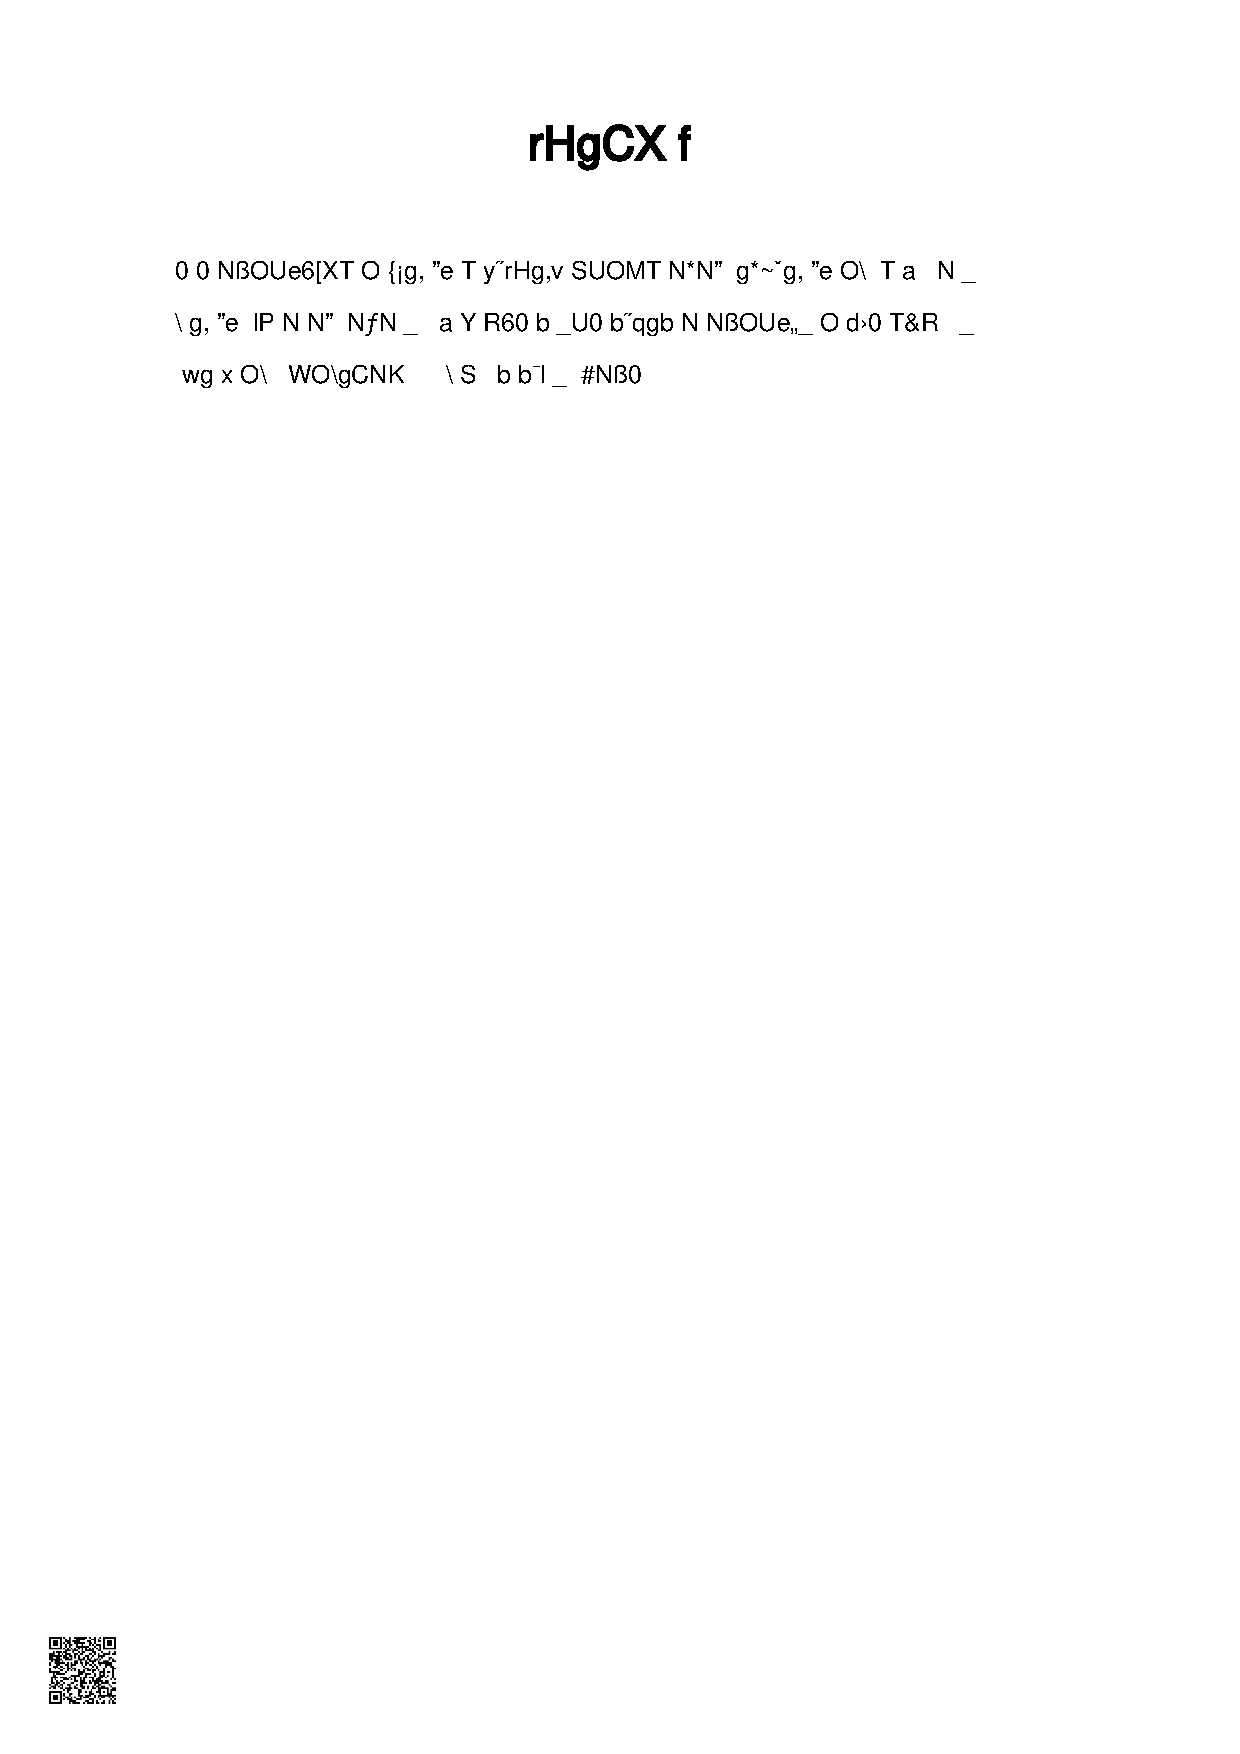
\includegraphics[height = 1.2448\textheight]{img/bqsm_180xxxxxxx.pdf}
    }
\end{textblock}

% vim:ts=4:sw=4

	\cleardoublepage
	\pagestyle{plain}
	\setcounter{page}{0}
	\pagenumbering{Roman}
	\begin{cabstract}
如课业目标所示,学生在第一章为论文精读选择 Increasing Controllable Oxygen Ions to Improve Device Performance Using Supercritical Fluid Technique in ZnO-Based Resistive Random Access Memory 为来源进行阅读,其因有三,第一在于与自己的博士研究方向相关,其二这是由台湾团队所出得研究成果,最后该篇研究成果为引用了我的导师张冠张老师曾经发表过的文章。第二章为考核为找到 100 篇文章进行处理,最后用表格整理本作业所搜集的文献。

\end{cabstract}

%\begin{eabstract}
%    英文摘要部分...
%\end{eabstract}

% vim:ts=4:sw=4

	\tableofcontents
	% 如有需要使用主要符号对照表
	\begin{denotation}

\item[$x,y,m,n,t$] 标量,通常为变量
\item[$K,L,D,M,N,T$] 标量,通常为超参数
\item[$x\in \mathbb{R}^{D}$] D维列向量
\item[$(x_1,\cdots,x_D)$] D维行向量
\item[$(x_1,\cdots,x_D)^T$ or $(x_1;\cdots;x_D)^T$]  D维行向量
\item[$x\in \mathbb{R}^{KD}$]  ($KD$)维的向量
\item[$\mathbb{M}_i$ or $\mathbb{M}_i(\v x)$]  第$i$列为$\v 1$(或者$\v x$),其余为$\v 0$的矩阵
\item[$diag(\v x)$]  对角矩阵,其对角元素为$\v x$
\item[$\v I_N$ or $I$]  ($N\times N$)的单位阵
\item[$\v A \in \mathbb{R}^{D_1\times D_2\times \cdots \times D_K}$]  大小为$D_1\times D_2\times \cdots \times D_K$的张量
\item[$\{x^{(n)}\}^{N}_{n=1}$]  集合
\item[$\{(x^{(n)},y^{(n)})\}^{N}_{n=1}$]  数据集
\item[$\mathcal{N}(\v x;\mu,\sum)$]  变量$x$服从均值为$\mu$,方差为$\sum$的高斯分布

\end{denotation}

\footnotetext[1]{本符号对照表内容选自\citeauthor{qiu2020nndl}老师的《神经网络与深度学习》\cite{qiu2020nndl}一书。}


	\mainmatter
	\chapter{论文精读}
\label{chap:1}

从下面两处期刊来源,进行翻译、阅读并写出心得,而研究论文来源如下所示 :
% \cite{garcia2020admd}
\begin{Verbatim}
1. IEEE Transactions on Pattern Analysis and Machine Intelligence
(TPAMI) (SCI IF 16.389), 2021.
2. IEEE Journal on Selected Areas in Communications (SCI IF 9.114), 2021.
\end{Verbatim}

而论文心得必须根据 IMRAD 的方式进行撰写,其流程分别为四部分,分别为前言(Introduction)、方法(Methods)、结果(Results)和讨论(Discussion),最后则是根据原论文架构的范例。

\section{论文精读资讯}

下列论文资讯有二 \cite{garcia2020admd} ,其一为 arXiv 的 1810.08437 所示 的资讯,其二为 IEEE Transactions on Pattern Analysis and Machine Intelligence 的公开资讯。

\begin{Verbatim}
Increasing Controllable Oxygen Ions to Improve Device Performance Using 
Supercritical Fluid Technique in ZnO-Based Resistive Random Access Memory
在 ZnO 基电阻随机存取存储器中使用超临界流体技术增加可控氧离子以提高器件性能

Sheng-Yao Chou, Chih-Cheng Yang, Ting-Chang Chang , Fellow, IEEE, Tsung-Ming Tsai , 
Shih-Kai Lin, Chan-Wei Kuo, Chung-Wei Wu, Yu-Bo Wang, and Simon M. Sze, Life Fellow, IEEE
\end{Verbatim}


\section{论文心得}

该心得则根据 IMRAD 的方法来分析。

\subsection{前言}

电阻随机存取存储器(RRAM)将在不久的将来取代闪存成为主流的非易失性存储器。某些显著的优势,如简单的金属-绝缘体-金属结构、低功耗和高速,使RRAM成为最适合集成电路的产品。过去,各种金属氧化物材料,如 Ta2O5、HfO2 和 NiO 已被用作 RRAM 的中间层。除这些材料外,具有优异电阻开关(RS)特性的ZnO也已用于RRA应用。基于价态变化机制解释了氧化锌基RRAM中的RS机制。

通过在电极上施加不同的极性电位来确定导电细丝(CF)的断裂和形成,导电细丝由开关层内的氧空位和间隙氧离子组成。氧离子通过电势迁移引起CF附近的氧化还原反应,从而触发CF电阻的变化。因此,控制CF附近的氧离子在RRAM的性能中起着关键作用。在先前的研究中,开关层中氧离子的不同浓度导致了器件性能的提高。在一些研究中,引入了氧气储层以提高设备性能。该层通常是一种氧化物绝缘体,具有高浓度的氧离子和用于储存铜绿氧的空位。

在其他研究中,氧环境的各种含量被诱导导致氧化物绝缘体中氧离子和空位的浓度增加。此外,还应用了一种新的超临界流体(SCF)处理方法来改进RRAM装置。具有高渗透性和高溶解性的SCF可以容易地渗透到器件中。因此,一些研究使用插入水分子的超临界CO2流体来改善绝缘性能。然而,在本研究中,不需要在绝缘体中充入更多氧气或插入其他材料。该装置在制造过程中采用高压纯超临界CO2流体处理。高压超临界CO2流体,无毒且稳定的化学特性可以渗透到纳米尺度结构中。由于这些优异的特性,超临界CO2流体可以显著削弱Zn-O键合,导致氧离子含量增加,而不改变原始元素比例。因此,超临界CO2流体技术是用于制备提高氧化锌基RRAM的RS性能的合适物质。在本研究中,超临界CO2流体处理因其优异的物理性质而被提出。为了研究其对ZnO开关层增加氧离子和改善氧化锌基RRAM的影响,在处理前后进行了电测量和材料分析。此外,通过实验证明了物理模型在提高器件性能方面的有效性。


\subsection{方法}

两组实验样品的制造工艺流程方法如论文图中所示。1.首先,使用原子层沉积在两个图案化的Ti/SiO2/Si衬底上沉积200nm氮化钛(TiN)作为底部电极。接下来,在这两个器件中,通孔的尺寸为1μm2,通过应用掩模对准进行图案化。10nm ZnO薄膜作为RRAM器件的开关层,通过在4mTorr的工作压力下使用30sccm Ar气体溅射ZnO靶来沉积。使用N\&K 1280分析仪测量ZnO薄膜的厚度。随后,一个样本被引入SCF过程。SCF系统和处理步骤如图所示。2.将样品置于反应室中,在80℃下加热◦C、 CO2由注射泵压缩至4000 psi,并引入反应室以达到临界点。CO2进入SCF状态后,样品进行1小时处理。处理后,在移除样品之前,将腔室减压至1大气压。最后,通过直流溅射沉积了200nm铂(Pt)作为两个样品的顶部电极。为了识别ZnO薄膜中的差异。(图2说明.SCF处理系统和处理步骤)在SCF处理之后,在Si晶片上制备未经处理和处理的10nm ZnO薄层用于材料分析。为了识别SCF处理后ZnO薄膜的差异,在Si晶片上制备了未经处理和处理的10nm ZnO薄膜用于材料分析。用JEOL JAMP-9500F Auger 电子能谱仪对材料进行了X射线光电子能谱(XPS)分析。电流-电压(I−五) 用 Agilent B1500A半导体参数分析仪和Cascade M150微探针站在室温和环境大气中进行电测量,以观察处理和未处理的RRAM的RS特性。向底部电极(TiN)施加直流电压,顶部电极(Pt)接地。

\subsection{结果}

SCF处理后,基于氧化锌的RRAM表现出更高的特性,包括更低的形成电压、更低的设定电压和更大的存储窗口。基于XPS分析,SCF处理后,开关层中的氧离子浓度增加,导致RS期间更剧烈的氧化反应。SCF技术可以被认为是提高RRAM设备中选择作为绝缘体的各种氧化物基材料中氧离子含量的有效方法。这种SCF技术加速了高性能RRAM器件的发展。

\subsection{讨论}

基于电流拟合和材料分析的结果,提出了处理和未处理装置的模型,在最后一图8.超临界CO2流体渗透到由于Zn-O键的弱化,导致更多的氧离子。SCF处理后,经处理的ZnO基RRAM可以在其氧化锌开关层中存储更多的氧离子,这提高了操作期间离子的可控性。因此,经处理的器件具有更好的RS特性,较低的形成电压、较小的VSET和较大的存储器窗口。由于更多的接近CF的氧离子参与氧化还原反应,肖特基距离和势垒高度比未处理的器件大,导致处理后的器件具有更大的HRS电阻和阻变储存的窗口区间。

\section{论文翻译}

在此根据论文 Increasing Controllable Oxygen Ions to Improve Device Performance Using Supercritical Fluid Technique in ZnO-Based Resistive Random Access Memory  的章节结构进行翻译,其论文题目的中文字面意义上为在 ZnO 基电阻随机存取存储器中使用超临界流体技术增加可控氧离子以提高器件性能 。该根据原研究论文架构来分配章节。

\subsection{摘要}
%Abstract 摘要

在这项研究中,提出了一种先进的超临界流体 (SCF) 技术,适用于低温 ( 80度C ) 和高压 (4000 psi) 的材料和电子设备,用于基于 ZnO 的电阻式随机存取存储器 (RRAM) )。在 SCF 处理后,X 射线光电子能谱 (XPS) 分析证实氧化锌薄膜中氧离子的浓度增加。此外,电学测量证实,与未经处理的器件相比,经处理的 ZnO 基随机存取存储器具有较低的形成电压、较低的置位电压和较高的高低阻态比率。接下来,通过拟合电流-电压曲线来研究载流子传输机制。最后,引入物理模型来说明额外的氧离子,这些氧离子在 SCF 处理后在随机存取存储器中产生更好的记忆特性。这种重要的 SCF 技术在不改变原始元素比例的情况下增加了氧离子的含量,并保持了简单的器件结构。因此,该技术显示出可行的材料改进潜力,能够在不久的将来进行有效的实际应用。

\subsection{前言}
% 1 INTRODUCTION 前言

电阻式随机存取存储器(RRAM)将在不久的将来取代 FLASH 存储器成为主流的非易失性存储器[1]-[7]。诸如简单的金属-绝缘体-金属结构、低功耗和高速等显着优势使 RRAM 最适合集成电路 [8]-[12]。过去,各种金属氧化物材料如 Ta2O5、HfO2 和 NiO 已被用作 RRAM 的中间层 [13]-[21]。除了这些材料之外,具有优异电阻开关 (RS) 特性的 ZnO 也已用于 RRAM 应用 [22]-[24]。

基于价态变化机制解释了基于氧化锌的 RRAM 中的 RS 机制。由开关层内的氧空位和间隙氧离子组成的导电丝 (CF) 的断裂和形成是通过在电极上施加不同的极性电势来确定的。氧离子通过电势迁移在 CF 附近引起氧化还原反应,从而引发 CF 电阻的变化。因此,控制 CF 附近的氧离子在 RRAM [25]-[28] 的性能中起着关键作用。在之前的研究中,开关层中不同浓度的氧离子可以提高器件性能[29]、[30]。在一些研究中,氧储存层被诱导来改善器件性能。该层通常是氧化物绝缘体,具有高浓度的氧离子和空位,用于储存过量的氧气[31]-[33]。
在其他研究中,各种氧环境含量被诱导导致氧化物绝缘体中氧离子和空位浓度的增加[34]-[36]。

此外,还应用了一种新型的超临界流体(SCF)处理来改进 RRAM 器件。SCF具有高渗透性和高溶解性,很容易渗透到设备中。因此,一些研究使用插入水分子的超临界 CO2 流体来改善绝缘体性能 [30]、[37]、[38]。然而,在这项研究中,不需要在绝缘体中充气更多的氧气或插入另一种材料。该装置在制造过程中采用高压纯超临界CO2流体处理。无毒、化学特性稳定的高压超临界CO2流体可以渗透到纳米级结构中。凭借这些优异的特性,超临界 CO2 流体可以显着削弱 Zn-O 键,导致氧离子含量增加而不改变原始元素比例。因此,超临界 CO2 流体技术是一种合适的物质,可应用于制造以改善氧化锌基 RRAM 的 RS 性能。在本研究中,由于其优异的物理性能,提出了超临界 CO2 流体处理。为了研究其对 ZnO 开关层增加过量氧离子和改善氧化锌基 RRAM 的影响,在处理前后进行了电测量和材料分析。此外,还进行了实验以证明物理模型在提高设备性能方面的有效性。


\begin{figure}[htb]
\centering 
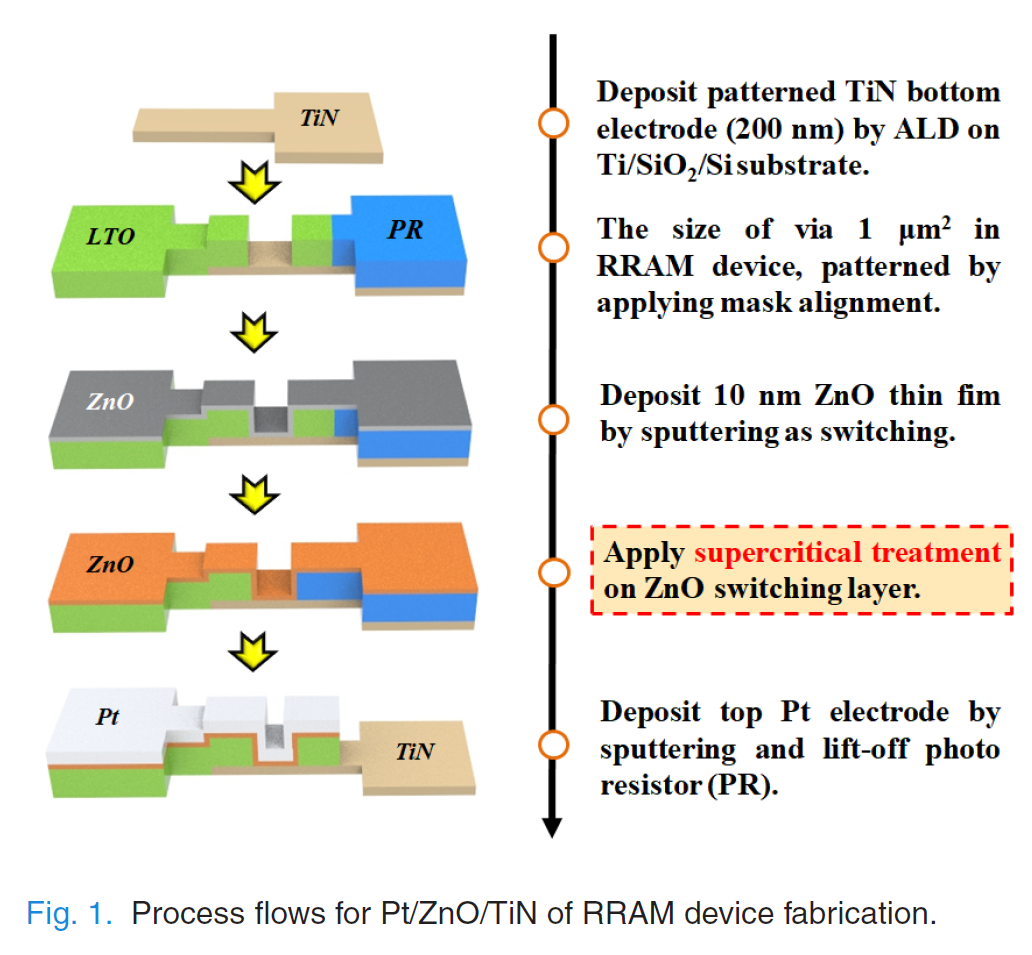
\includegraphics[width=0.80\textwidth]{img/c1m1.png} 
\caption{论文图 1}
\label{Test}
\end{figure}

图 1. RRAM 器件制造的 Pt/ZnO/TiN of RRAM 工艺流程。

\subsection{实验装置}
% 2 EXPERIMENTS 实验

两个实验样品的制造工艺流程如图1所示。首先,使用原子层沉积在两个图案化的 Ti/SiO2/Si 衬底上沉积 200 nm 氮化钛 (TiN) 作为底部电极。接下来,在这两个器件中,通孔的尺寸为 1 μm2,通过应用掩模对准进行图案化。10 nm ZnO 薄膜作为 RRAM 器件的开关层,通过使用 30 sccm Ar 气体在 4 mTorr 的工作压力下溅射 ZnO 靶材而沉积。使用 N\&K 1280 分析仪测量 ZnO 薄膜的厚度。随后,将其中一个样品引入 SCF 工艺。SCF 系统和处理步骤如图 2 所示。将样品置于反应室中,加热至 80 摄氏度。CO2 被注射泵压缩至 4000 psi 并引入反应室以达到临界点。CO2 进入 SCF 状态后,样品进行 1 h 处理。

\begin{figure}[htb]
\centering 
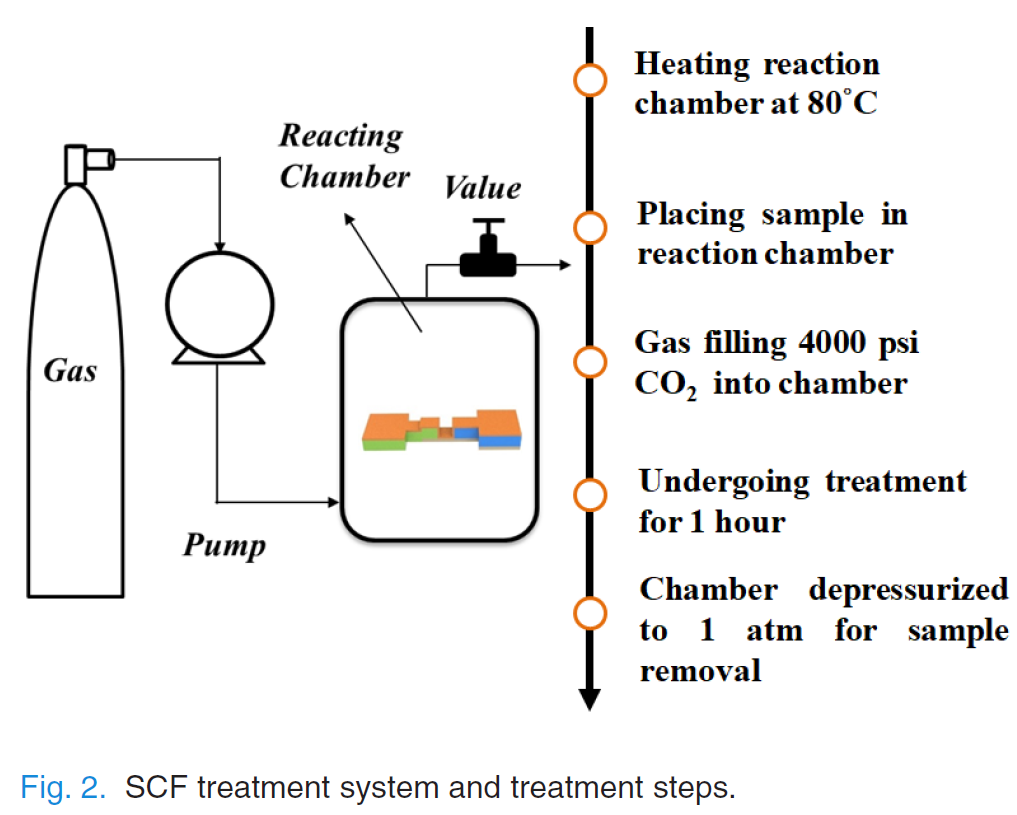
\includegraphics[width=0.80\textwidth]{img/c1m2.png} 
\caption{论文图 2}
\label{Test}
\end{figure}

图 2 SCF 处理系统和处理步骤。

处理后,在取出样品之前将腔室减压至 1 个大气压。最后,随后通过直流溅射沉积作为两个样品的顶部电极的 200 nm 铂 (Pt)。为了识别 SCF 处理后 ZnO 薄膜的差异,制备了 Si 晶片上未经处理和处理的 10 nm ZnO 薄膜用于材料分析。为了识别 SCF 处理后 ZnO 薄膜的差异,制备了 Si 晶片上未经处理和处理的 10 nm ZnO 薄膜用于材料分析。X射线光电子能谱(XPS)的材料分析是通过JEOL JAMP-9500F俄歇电子能谱仪获得的。使用 Agilent B1500A 半导体参数分析仪和 Cascade M150 微探针台在室温和环境大气中进行电流 - 电压 (I - V) 电气测量以观察处理和未处理 RRAM 的 RS 特性。直流电压提供给底部电极 (TiN),顶部电极 (Pt) 接地。

\subsection{结果与讨论}
% 3 RESULTS AND DISCUSSION 结果与讨论

为了证明 SCF 处理对器件的影响,对经过处理和未经处理的器件进行了 XPS 分析,如图 3 所示。如图 3(a) 中的宽扫描 XPS 光谱所示,处理和未处理的 ZnO 薄膜的成分几乎相同 [39]-[42]。此外,对 ZnO 薄膜的 O 1 s 峰进行去卷积,以观察氧原子的不同状态。531.8 和 529.9 eV 处的去卷积峰分别与氧离子对键合缺陷的贡献和氧原子与 Zn 原子的键合有关[43]-[46]。图 3(b)和(c)表明 SCF 处理后 Zn-O 键合的百分比显着降低。相比之下,氧离子的比例从29\%增加到77\%。

基于 XPS 分析,SCF 处理通过增加用于切换的可控氧离子来改善 ZnO 层中的切换层。图 4 显示了处理和未处理器件的开关特性。在切换器件之前,施加形成电压以激活切换特性。100μA 顺从电流下成形特性的双扫描 IV 曲线如图 4(a) 所示。蓝色和绿色箭头分别表示前向和后向扫描。后向扫描在成形过程后呈现导通状态电流。

\begin{figure}[htb]
\centering 
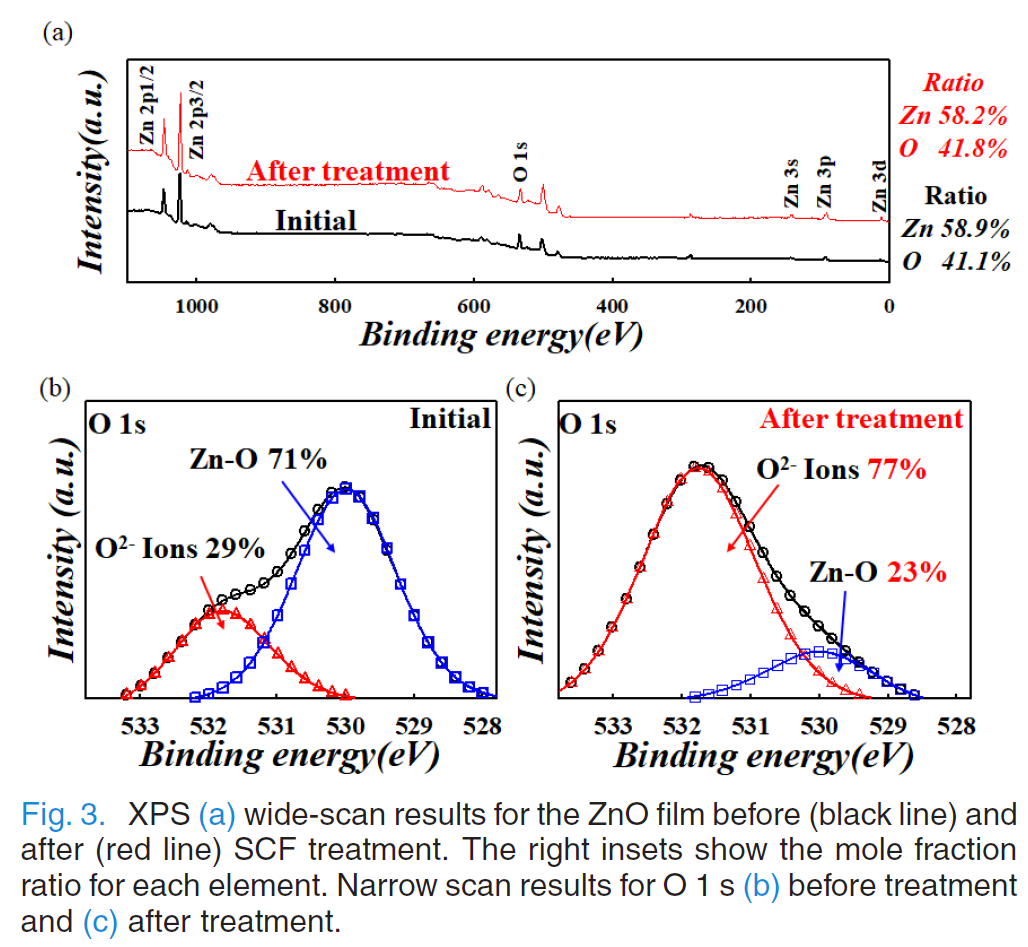
\includegraphics[width=0.80\textwidth]{img/c1m3.png} 
\caption{论文图 3}
\label{Test}
\end{figure}

图 3.SCF 处理之前(黑线)和之后(红线)ZnO 薄膜的 XPS(a)宽扫描结果。右侧插图显示了每种元素的摩尔分数比。O 1 s (b) 治疗前和 (c) 治疗后的窄扫描结果。



\begin{figure}[htb]
\centering 
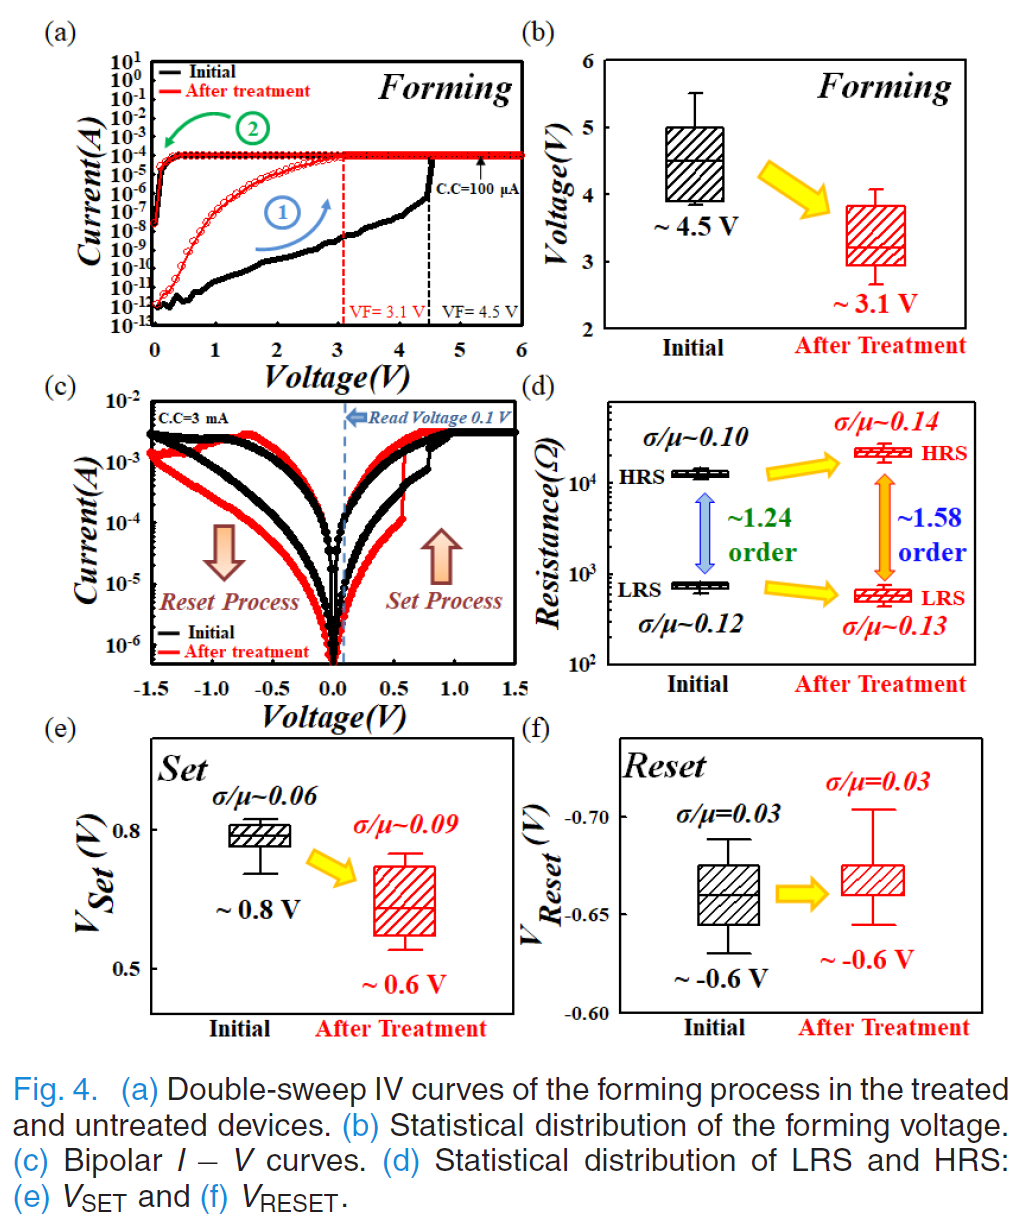
\includegraphics[width=0.80\textwidth]{img/c1m4.png} 
\caption{论文图 4}
\label{Test}
\end{figure}
图 4. (a) 处理和未处理器件成型过程的双扫描 IV 曲线。(b) 成型电压的统计分布。(c) 双极 I - V 曲线。(d) LRS 和 HRS 的统计分布:(e) VSET 和 (f) VRESET。

因此,当电流达到 100 μA 的顺从电流时,正向扫描中验证了 3.1 和 4.5 V 的形成电压。与未经处理的器件相比,经处理的器件的成型电压从 4.5 V 提高到 3.1 V。由于 SCF 处理增加了氧空位和氧离子,更多的导电路径导致形成电压降低。此外,收集十个随机点进行静态验证,以验证两种器件的形成电压的变化,如图4(b)所示。

未经处理的器件的平均形成电压约为 4.5 V。相比之下,处理后的器件表现出约 3.1 V 的较低平均形成电压,表明 SCF 处理有效地改善了形成电压的降低。在形成过程之后,器件的电阻状态可以通过不同极性的电位来切换。

当底部电极受到正偏压时,器件会经历一个设置过程,并由于 CF 的形成而从高阻态 (HRS) 切换到低阻态 (LRS)。相反,当向底部电极施加负偏压时,器件会经历复位过程,并由于 CF 的破裂而从 LRS 切换到 HRS。处理和未处理器件的开关特性如图4(c)所示。

I - V 扫描在设置过程中以 1.5 V 偏置和 3 mA 顺从电流在器件上运行,在复位过程中使用 -1.5 V 负偏置。增加氧离子和空位以改善 CF 曲线会导致更高的导通状态电流和更低的关断状态电流。

改善了设备处理后的设定电压和内存窗口,使设备功耗和设备RS的识别分别更低和更容易。此外,收集了一个设备中的多个周期进行统计分析,以验证两个设备的 RS 特性和 VSET/VRESET 的变化,如图 4(d)-(f) 所示。

处理后的器械中 HRS 和 LRS 的比率为 1.6 个数量级,而未处理的器械中的比率为 1.2 个数量级,远低于处理过的器械。此外,提取两个设备的变化系数 (CV) 以验证变化。

两种设备中 LRS 和 HRS 的 CV 相似。VSET/VRESET 如图 4(e) 和 (f) 所示。经过处理的设备的 VSET 比未经处理的设备低 0.8 倍。
经处理和未经处理的装置中 VSET 的 CV 分别为 0.06 和 0.09。两个器件中 VRESET 的 CV 均为 0.03。

处理过的设备中 VSET 的 CV 大于未处理过的设备。先前的一项研究还表明,由于氧离子的比例较高,在 ZnO 基开关层中观察到 VSET 的较大变化和较小的 VRESET 变化 [47]。在这项工作中,根据图 3 所示的 O 1 s XPS 结果,SCF 处理后氧离子的含量增加。切换层中更多的氧离子可用于设置过程。
因此,建议的处理后设定电压降低。

然而,氧离子的增加也会导致设定过程中工作电压的较大变化。此外,HRS 和 LRS 分布都证实了在所提出的处理后可以获得更高的内存窗口,这表明 SCF 技术是基于实验结果改进 RRAM 器件的有效方法。对于处理和未处理装置的均匀性,测量了五个未处理和五个具有相同结构的处理装置的多个 HRS/LRS/VSET/VRESET 循环的相应统计分布,如图 5 所示。

两种器件在 HRS/LRS/VSET/VRESET 方面均表现出良好的一致性。与未处理的设备相比,所有处理过的设备都具有更大的内存窗口,如图 5(a)和(b)所示。此外,所有处理过的设备都表现出比未经处理的设备更低的 VSET 值,如图 5(c)和(d)所示。两种器件中的 VRESET 相似,如图 5(e) 和 (f) 所示。

因此,SCF技术是提高RRAM器件性能的有效方法。对于实际内存应用,两种器件的耐用性和保持性都被用来研究它们的可靠性,如图 6 所示。在图 6(a) 和 (b) 中,经处理和未经处理的装置在耐久试验中至少可操作 105 次。此外,在图 6(c)和(d)所示的保持测试中,它们的电阻状态能够保持至少 104 秒而没有任何退化。此外,处理过的设备表现出更大的内存窗口。两种器件中 HRS 的载流子传输机制均以肖特基机制为主。肖特基发射方程可以表示为

$$
J=A^{* *} T^2 \exp \left[\frac{-q\left(\phi_B-\sqrt{q V / 4 \pi \varepsilon_i d_{\mathrm{sch}}}\right.}{k_B T}\right]
$$
其中 $\mathrm{A}^{* *}$、$\varepsilon_i$ 和 $\varphi_B$ 分别是有效理查森常数、绝缘体介电常数和势垒高度 [48]。
图中斜率和截距的物理意义可以通过计算肖特基方程的对数。

% where $\mathrm{A}^{* *}$, $\varepsilon_i$, and $\varphi_B$ are the effective Richardson constant, insulator permittivity, and barrier height, respectively [48].

% The physical meaning of the slope and intercept in a $\ln \left(\mathrm{J} / \mathrm{T}^2\right)-\mathrm{V}^{0.5}$ plot can be verified by calculating the logarithm of the Schottky equation. 
$\ln \left(\mathrm{J} / \mathrm{T}^2\right)-\mathrm{V}^{0.5}$ 
% The slope and intercept are dependent on the barrier height and the Schottky distance, respectively, because the slope and intercept are proportional to $\left(\left(1 / \varepsilon_i d\right)\right)^{1 / 2}$ and $\varphi_B$, respectively, where d is the Schottky distance. 
斜率和截距分别取决于势垒高度和肖特基距离,因为斜率和截距与 $\left(\left(1 / \varepsilon_id\right)\right)^{1 / 2}$ 成正比和 $\varphi_B$,其中 d 是肖特基距离。图 7(a) 和 (b) 表明两种器件的 HRS 均受肖特基机制支配。

此外,处理后的器件具有较大的截距和斜率,对应于其较大的势垒高度和肖特基距离。基于当前拟合和材料分析的结果,提出了处理和未处理设备的模型,如图 8 所示。超临界 CO2 流体渗透到 ZnO 纳米结构中,由于 Zn-O 键合减弱而导致更多的氧离子。

经过SCF处理后,处理后的ZnO基RRAM可以在其氧化锌开关层中储存更多的氧离子,提高了运行过程中离子的可控性。
因此,处理后的器件具有较好的RS特性,例如较低的形成电压、较小的VSET和较大的存储窗口。
由于CF附近更多的氧离子参与氧化还原反应,因此肖克蒂距离和势垒高度比未处理的器件大,使得处理后的器件具有更大的HRS电阻和更好的记忆窗口。







\begin{figure}[htb]
\centering 
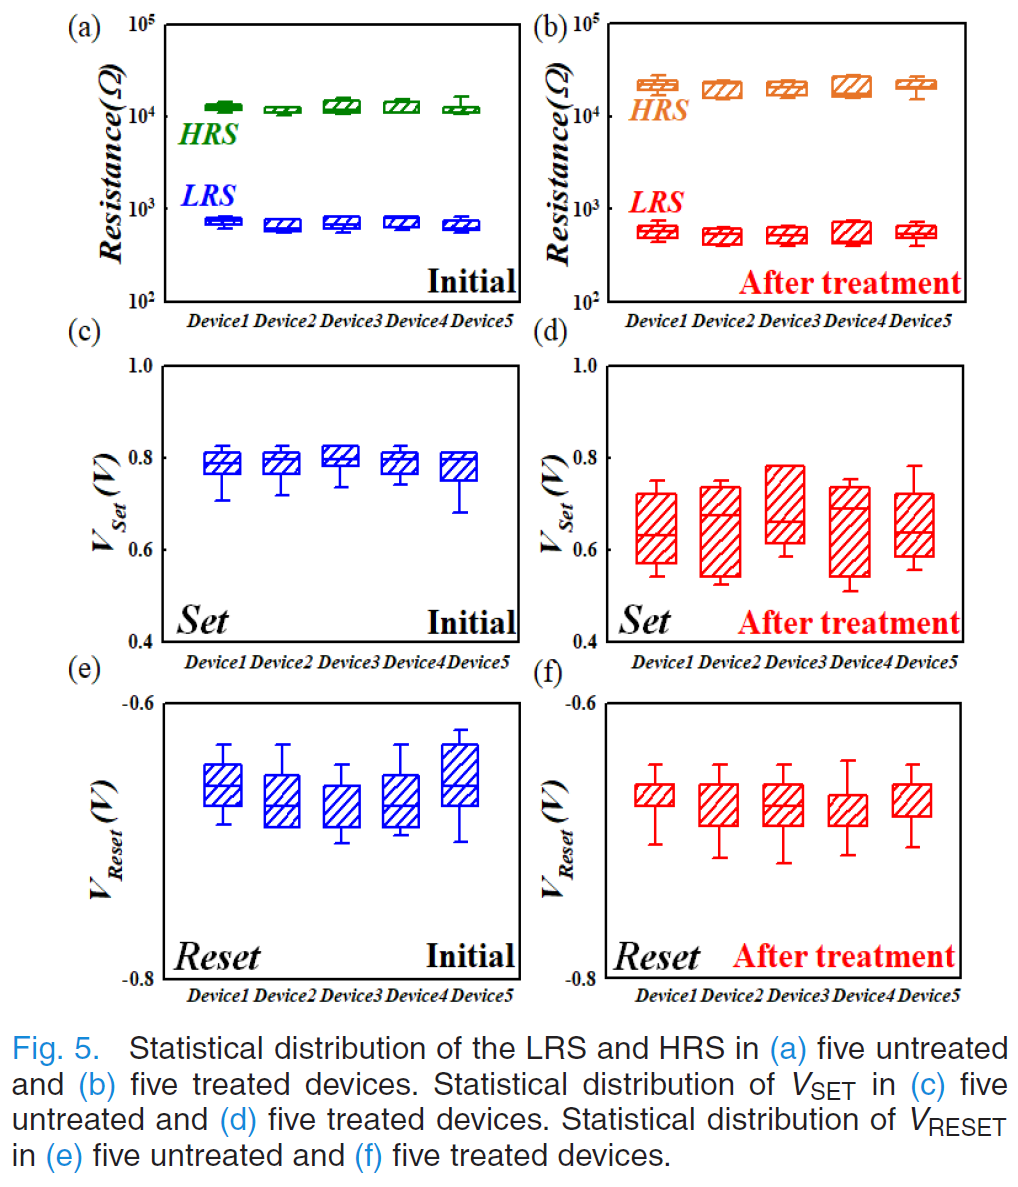
\includegraphics[width=0.80\textwidth]{img/c1m5.png} 
\caption{论文图 5}
\label{Test}
\end{figure}
图 5。LRS 和 HRS 在(a)五个未处理和(b)五个处理设备中的统计分布。VSET 在(c)五个未处理和(d)五个处理设备中的统计分布。VRESET 在(e)五个未处理和(f)五个处理过的设备中的统计分布。

\begin{figure}[htb]
\centering 
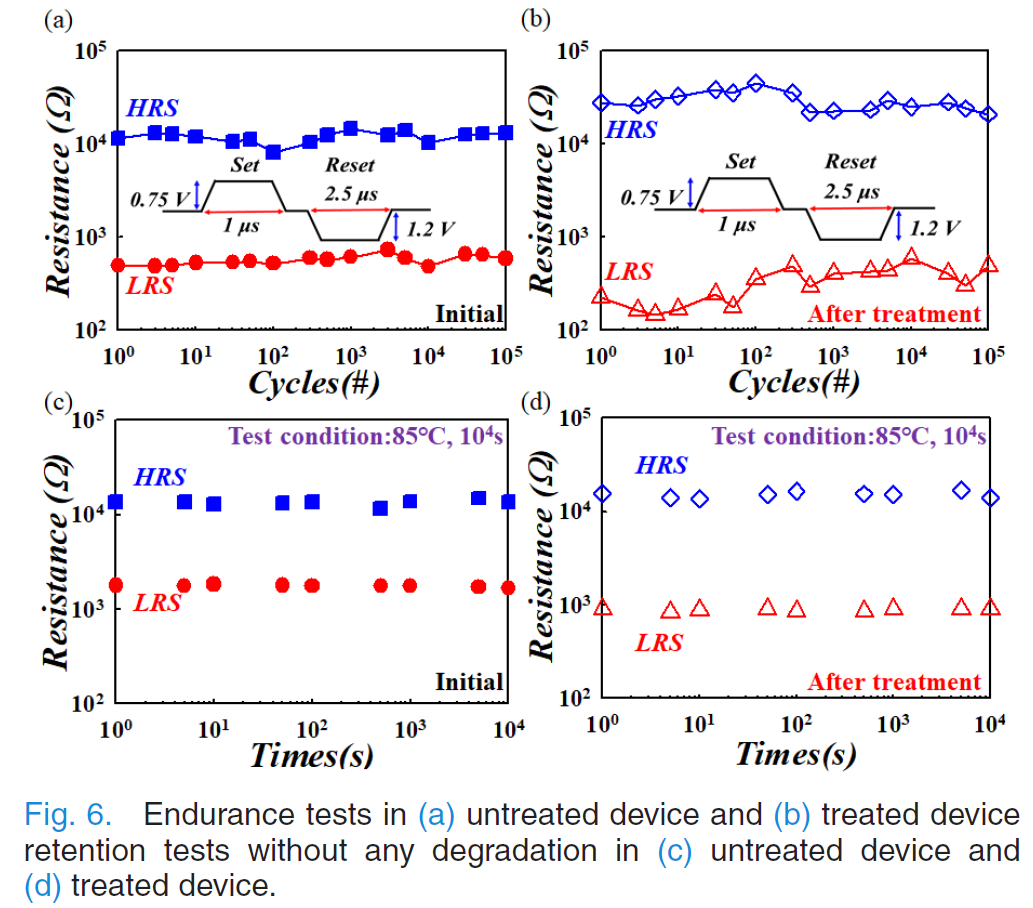
\includegraphics[width=0.80\textwidth]{img/c1m6.png} 
\caption{论文图 6}
\label{Test}
\end{figure}
图 6. (a) 未处理设备和 (b) 处理设备保持测试的耐久性测试,(c) 未处理设备和 (d) 处理设备没有任何退化。

\begin{figure}[htb]
\centering 
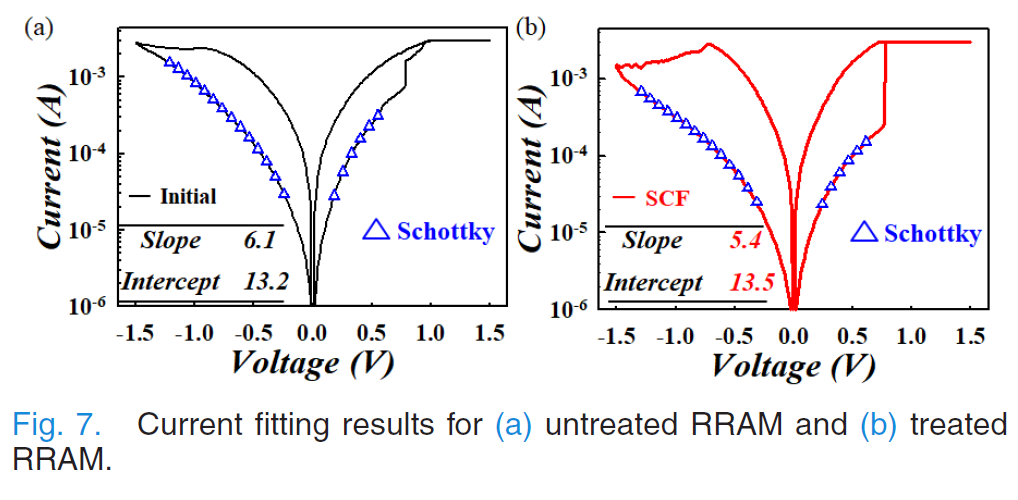
\includegraphics[width=0.80\textwidth]{img/c1m7.png} 
\caption{论文图 7}
\label{Test}
\end{figure}
图 7. (a) 未处理的 RRAM 和 (b) 处理的 RRAM 的当前拟合结果。

\begin{figure}[htb]
\centering 
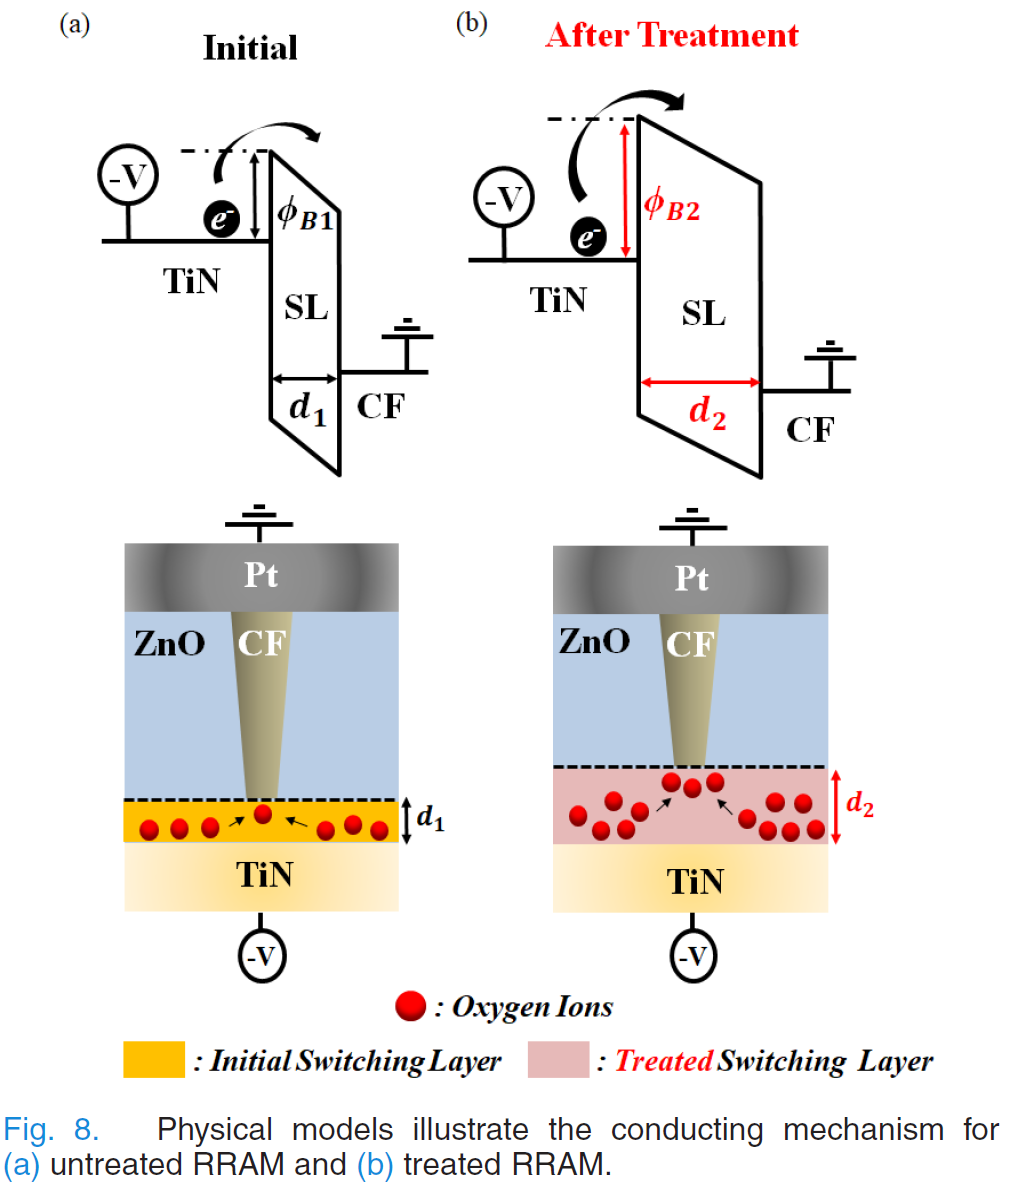
\includegraphics[width=0.80\textwidth]{img/c1m8.png} 
\caption{论文图 8}
\label{Test}
\end{figure}
图 8. 物理模型说明了 (a) 未处理的 RRAM 和 (b) 处理的 RRAM 的传导机制。


%\begin{itemize}
%\item Calculus
%\item Linear Algebra
%\item Basic Computer Concepts
%\end{itemize}

%\begin{description}
% \item[First] \hfill \\
% The first item
% \item[Second] \hfill \\
% The second item
% \item[Third] \hfill \\
% The third etc \ldots
%\end{description}

\subsection{结论}
% 4 CONCLUSIONS 结论

经过SCF处理后,氧化锌基RRAM表现出更好的特性,包括更低的形成电压、更低的置位电压和更大的存储窗口。基于 XPS 分析,SCF 处理后开关层中的氧离子浓度增加,导致 RS 期间的氧化还原反应更加剧烈。SCF 技术可以被认为是一种有效的方法来增加各种氧化物基材料中氧离子的含量,这些材料被选为 RRAM 器件中的绝缘体。这种 SCF 技术加速了高性能 RRAM 器件的开发。


	\chapter{参考文献搜集}

下列为本次作业所搜集而来的文献表,根据本次作业的 7 项来源进行搜集,其包括 IEEE Transaction/Magazine/Journal、IET (IEE) Proceeding/Magazine/Journal、ACM、Springer、Elsevier、Google 学术、Beidu 学术等,最后明确标示使用的平台搜寻引擎跟文献年份。

\begin{center}
\begin{tabular}{cccc}
\hline
研究者 & 平台 & 来源分类 & 备注年份  \\
\hline
Yingkun Xu et al. \cite{yingkunxu2019} & Baidu Scholar & IET (IEE) Proceeding & 2019 \\
Qin Wu et al. \cite{qinwu2020} & Baidu Scholar & IET (IEE) Proceeding & 2020 \\
Abimael Guzmán Pando et al. \cite{abimael2020} & Baidu Scholar & IET (IEE) Proceeding & 2020 \\
Sarah Ahmed et al. \cite{sarahahmed2020} & Baidu Scholar & IET (IEE) Proceeding & 2020 \\
Francisco Luongo et al. \cite{franciscoluongo2020} & Baidu Scholar & IET (IEE) Proceeding & 2020 \\
\hline
\end{tabular}
\end{center}

\begin{center}
\begin{tabular}{cccc}
\hline
研究者 & 平台 & 来源分类 & 备注年份  \\
\hline
Huiyun Gong et al. \cite{huiyungong2021} & Google Scholar & IET (IEE) Proceeding & 2021 \\
Iman Iraei et al. \cite{imaniraei2021} & Google Scholar & IET (IEE) Proceeding & 2021 \\
Yuling Xing et al. \cite{yulingxing2021} & Google Scholar & IET (IEE) Proceeding & 2021 \\
Na Zhu et al. \cite{nazhu2021} & Google Scholar & IET (IEE) Proceeding & 2021 \\
Mohammad Ali Amirabadi et al. \cite{mohammadaliamirabadi2021} & Google Scholar & IET (IEE) Proceeding & 2021 \\
Yanlin Wu et al. \cite{yanlinwu2021} & Google Scholar & IET (IEE) Proceeding & 2021 \\
Jiawei Nian et al. \cite{jiaweinian2021} & Google Scholar & IET (IEE) Proceeding & 2021 \\
Zhao Zhen et al. \cite{zhaozhen2021} & Google Scholar & IET (IEE) Proceeding & 2021 \\
Olarewaju Mubashiru Lawal et al. \cite{olarewaju2021} & Google Scholar & IET (IEE) Proceeding & 2021 \\
Guanwen Zhang et al. \cite{guanwenzhang2021} & Google Scholar & IET (IEE) Proceeding & 2021 \\
Azka Wani et al. \cite{azkawani2021} & Google Scholar & IET (IEE) Proceeding & 2021 \\
Hongxin Ji et al. \cite{hongxinji2021} & Google Scholar & IET (IEE) Proceeding & 2021 \\
Junpeng Wu et al. \cite{junpengwu2021} & Google Scholar & IET (IEE) Proceeding & 2021 \\
Chengxu Ma et al. \cite{chengxuma2021} & Google Scholar & IET (IEE) Proceeding & 2021 \\
Mukesh Kumar Tripathi et al. \cite{mukeshkumar2021} & Google Scholar & IET (IEE) Proceeding & 2021 \\
\hline
\end{tabular}
\end{center}

\begin{center}
\begin{tabular}{cccc}
\hline
研究者 & 平台 & 来源分类 & 备注年份  \\
\hline
Wei Liang et al. \cite{weiliang2021} & ACM & ACM Library & 2021 \\
Wu Q et al. \cite{wuq2021} & ACM & ACM Library & 2021 \\
Chiyuan Zhang et al. \cite{chiyuanzhang2021} & ACM & ACM Library & 2021 \\
Kaixuan Chen et al. \cite{kaixuanchen2021} & ACM & ACM Library & 2021 \\
Shervin Minaee et al. \cite{shervinminaee2021} & ACM & ACM Library & 2021 \\
Guansong Pang et al. \cite{guansongpang2021} & ACM & ACM Library & 2021 \\
Garvit Goel et al. \cite{garvitgoel2021} & ACM & ACM Library & 2021 \\
Tom van der Weide et al. \cite{tomvanderweide2017} & ACM & ACM Library & 2021 \\
Abdul Wasay et al. \cite{abdulwasay2021} & ACM & ACM Library & 2021 \\
Matthew Kusz et al. \cite{matthewkusz2021} & ACM & ACM Library & 2021 \\
\hline
\end{tabular}
\end{center}

\begin{center}
\begin{tabular}{cccc}
\hline
研究者 & 平台 & 来源分类 & 备注年份  \\
\hline
Hironobu Fujiyoshi et al. \cite{fujiyoshi2021} & ScienceDirect & Elsevier & 2021 \\
Geert Litjens PhD et al. \cite{geertlitjens2019} & ScienceDirect & Elsevier & 2019 \\
George Onoufriou et al. \cite{george2019} & ScienceDirect & Elsevier & 2019 \\
A.Inés et al. \cite{aines2019} & ScienceDirect & Elsevier & 2019 \\
Jihoon Oh et al. \cite{jihoonoh2019} & ScienceDirect & Elsevier & 2019 \\
\hline
\end{tabular}
\end{center}

\begin{center}
\begin{tabular}{cccc}
\hline
研究者 & 平台 & 来源分类 & 备注年份  \\
\hline
Carole H. Sudre et al. \cite{carole2017} & Springer & Springer Link & 2017 \\
Mohammad Hesam Hesamian et al. \cite{hesamian2019} & Springer & Springer Link & 2019 \\
Pim Moeskops et al. \cite{pimmoeskops2016} & Springer & Springer Link & 2016 \\
Niall O’Mahony et al. \cite{niall2019} & Springer & Springer Link & 2019 \\
Huazhu Fu et al. \cite{huazhufu2016} & Springer & Springer Link & 2016 \\
\hline
\end{tabular}
\end{center}

\begin{center}
\begin{tabular}{cccc}
\hline
研究者 & 平台 & 来源分类 & 备注年份  \\
\hline
Sarah Adel Bargal et al. \cite{sarahadel2021} & Google Scholar & IEEE Transactions & 2021 \\
Xu Yang et al. \cite{xuyang2021} & Google Scholar & IEEE Transactions & 2021 \\
Mingjie Sun et al. \cite{mingjie2021} & Google Scholar & IEEE Transactions & 2021 \\
Piotr Koniusz et al. \cite{piotr2021} & Google Scholar & IEEE Transactions & 2021 \\
Jianfeng Dong et al. \cite{jianfeng2021} & Google Scholar & IEEE Transactions & 2021 \\
Aysegul Dundar et al. \cite{aysegul2021} & Google Scholar & IEEE Transactions & 2021 \\
Yulin Wang et al. \cite{yulin2021} & Google Scholar & IEEE Transactions & 2021 \\
Lucas Zimmer et al. \cite{lucas2021} & Google Scholar & IEEE Transactions & 2021 \\
Maosen Li et al. \cite{maosen2021} & Google Scholar & IEEE Transactions & 2021 \\
Yang Zhang et al. \cite{yang2021} & Google Scholar & IEEE Transactions & 2021 \\
Kaiyang Zhou et al. \cite{kaiyang2021} & Google Scholar & IEEE Transactions & 2021 \\
Kai Zhao et al. \cite{kaizhao2021} & Google Scholar & IEEE Transactions & 2021 \\
Piotr Koniusz et al. \cite{piotrkoniusz2021} & Google Scholar & IEEE Transactions & 2021 \\
Wenguan Wang et al. \cite{wenguan2021} & Google Scholar & IEEE Transactions & 2021 \\
Xiangbo Shu et al. \cite{xiangbo2021} & Google Scholar & IEEE Transactions & 2021 \\
Wenguan Wang et al. \cite{tianfeizhou2021} & Google Scholar & IEEE Transactions & 2021 \\
Jun Ma et al. \cite{junma2021} & Google Scholar & IEEE Transactions & 2021 \\
Jibin Wu et al. \cite{jibinwu2021} & Google Scholar & IEEE Transactions & 2021 \\
Zhihua Wang et al. \cite{zhihuawang2021} & Google Scholar & IEEE Transactions & 2021 \\
Linjiang Huang et al. \cite{linjiang2021} & Google Scholar & IEEE Transactions & 2021 \\
Nicolas Gillis et al. \cite{nicolasgillis2021} & Google Scholar & IEEE Transactions & 2021 \\
Zhi-Hao Lin et al. \cite{zhihaolin2021} & Google Scholar & IEEE Transactions & 2021 \\
Guohao Li et al. \cite{guohaoli2021} & Google Scholar & IEEE Transactions & 2021 \\
Keren Fu et al. \cite{kerenfu2021} & Google Scholar & IEEE Transactions & 2021 \\
Elvin Isufi et al. \cite{elvinisufi2021} & Google Scholar & IEEE Transactions & 2021 \\
Yawei Luo et al. \cite{yaweiluo2021} & Google Scholar & IEEE Transactions & 2021 \\
Jiangliu Wang et al. \cite{jiangliuwang2021} & Google Scholar & IEEE Transactions & 2021 \\
Mehdi Ali et al. \cite{mehdiali2021} & Google Scholar & IEEE Transactions & 2021 \\
Lin Wang et al. \cite{linwang2021} & Google Scholar & IEEE Transactions & 2021 \\
Xiaosong Zhang et al. \cite{xiaosongzhangfangwan2021} & Google Scholar & IEEE Transactions & 2021 \\
\hline
\end{tabular}
\end{center}


\begin{center}
\begin{tabular}{cccc}
\hline
研究者 & 平台 & 来源分类 & 备注年份  \\
\hline
Filippo Maria Bianchi et al. \cite{filippo2021} & IEEE Xplore & IEEE Transactions & 2021 \\
Xingang Pan et al. \cite{xingang2021} & IEEE Xplore & IEEE Transactions & 2021 \\
Shervin Minaee et al. \cite{shervin2021} & IEEE Xplore & IEEE Transactions & 2021 \\
Xuan Zhang et al. \cite{xuan2021} & IEEE Xplore & IEEE Transactions & 2021 \\
Rui Zhang et al. \cite{rui2021} & IEEE Xplore & IEEE Transactions & 2021 \\
Hongyang Gao et al. \cite{hongyang2021} & IEEE Xplore & IEEE Transactions & 2021 \\
Kai Zhang et al. \cite{kai2021} & IEEE Xplore & IEEE Transactions & 2021 \\
Ke Yu et al. \cite{ke2021} & IEEE Xplore & IEEE Transactions & 2021 \\
Zilong Huang et al. \cite{zilong2021} & IEEE Xplore & IEEE Transactions & 2021 \\
Ming-Kun Xie et al. \cite{mingkun2021} & IEEE Xplore & IEEE Transactions & 2021 \\
Chaoyou Fu et al. \cite{chaoyou2021} & IEEE Xplore & IEEE Transactions & 2021 \\
Mang Ye et al. \cite{mang2021} & IEEE Xplore & IEEE Transactions & 2021 \\
Hongshuang Zhang et al. \cite{hongshuang2021} & IEEE Xplore & IEEE Transactions & 2021 \\
Hanqing Chao et al. \cite{hanqing2021} & IEEE Xplore & IEEE Transactions & 2021 \\
Zerong Zheng et al. \cite{zerong2021} & IEEE Xplore & IEEE Transactions & 2021 \\
Lei Cai et al. \cite{lei2021} & IEEE Xplore & IEEE Transactions & 2021 \\
Xuanyi Dong et al. \cite{xuanyi2021} & IEEE Xplore & IEEE Transactions & 2021 \\
Xinyu Chen et al. \cite{xinyu2021} & IEEE Xplore & IEEE Transactions & 2021 \\
Mathew Monfort et al. \cite{mathew2021} & IEEE Xplore & IEEE Transactions & 2021 \\
Deng-Ping Fan et al. \cite{dengping2021} & IEEE Xplore & IEEE Transactions & 2021 \\
Joey Tianyi Zhou et al. \cite{joeytianyi2021} & IEEE Xplore & IEEE Transactions & 2021 \\
Zhentao Tan et al. \cite{zhentao2021} & IEEE Xplore & IEEE Transactions & 2021 \\
Zhichao Lu et al. \cite{zhichao2021} & IEEE Xplore & IEEE Transactions & 2021 \\
Yi Liu et al. \cite{yi2021} & IEEE Xplore & IEEE Transactions & 2021 \\
Jie Mei et al. \cite{jie2021} & IEEE Xplore & IEEE Transactions & 2021 \\
Adnan Siraj Rakin et al. \cite{adnansiraj2021} & IEEE Xplore & IEEE Transactions & 2021 \\
Jiayuan Li et al. \cite{jiayuan2021} & IEEE Xplore & IEEE Transactions & 2021 \\
Gan Sun et al. \cite{gan2021} & IEEE Xplore & IEEE Transactions & 2021 \\
Jian Liang et al. \cite{jian2021} & IEEE Xplore & IEEE Transactions & 2021 \\
Deng-Bao Wang et al. \cite{dengbao2021} & IEEE Xplore & IEEE Transactions & 2021 \\
\hline
\end{tabular}
\end{center}




    
    \appendix
    \printbibliography[heading = bibintoc]
    
    % 如有需要使用研究生成果页
    \def\cpublication{攻读硕士期间发表的论文及其他成果}

%\renewcommand{\bibname}{\cpublication}
%\begin{thebibliography}{9}{
%\zihao{5}
%\bibitem{publish} 
%\textbf{扎克·施耐德}, XXX XXX, et al. XXXX Title[C/OL]//III H D, SINGH A. Proceedings of Machine Learning Research: Proceedings of the 37th International Conference on Machine Learning: vol. 119. [S.l.]: PMLR, 2020: XXXX-XXXX. http://proceedings.ml r.press/XXXX.html.(一作,CCF-A)
%}\end{thebibliography}
%\addcontentsline{toc}{chapter}{\cpublication}


	\backmatter
	\chapter{致谢}

非常感谢科技论文写作课的朱跃生教授,在科技论文写作课让学生上充分了解科技论文写作的知识与观念,同时又透过 Overleaf 平台实作了 LaTeX 的各类模板与写法,该流程也改善了自己目前的开发与研究工作模式,最后感谢在这一学期来一起读书得同学们跟室友对我这个资深同学的帮助。

	% 需替换门户原创页pdf/扫描pdf
	%% Copyright (c) 2008-2009 solvethis
% Copyright (c) 2010-2017,2021 Casper Ti. Vector
% Copyright (c) 2021 Kurapica
% Copyright (c) 2021 iofu728
% All rights reserved.
%
% Redistribution and use in source and binary forms, with or without
% modification, are permitted provided that the following conditions are
% met:
%
% * Redistributions of source code must retain the above copyright notice,
%   this list of conditions and the following disclaimer.
% * Redistributions in binary form must reproduce the above copyright
%   notice, this list of conditions and the following disclaimer in the
%   documentation and/or other materials provided with the distribution.
% * Neither the name of Peking University nor the names of its contributors
%   may be used to endorse or promote products derived from this software
%   without specific prior written permission.
%
% THIS SOFTWARE IS PROVIDED BY THE COPYRIGHT HOLDERS AND CONTRIBUTORS "AS
% IS" AND ANY EXPRESS OR IMPLIED WARRANTIES, INCLUDING, BUT NOT LIMITED TO,
% THE IMPLIED WARRANTIES OF MERCHANTABILITY AND FITNESS FOR A PARTICULAR
% PURPOSE ARE DISCLAIMED. IN NO EVENT SHALL THE COPYRIGHT HOLDER OR
% CONTRIBUTORS BE LIABLE FOR ANY DIRECT, INDIRECT, INCIDENTAL, SPECIAL,
% EXEMPLARY, OR CONSEQUENTIAL DAMAGES (INCLUDING, BUT NOT LIMITED TO,
% PROCUREMENT OF SUBSTITUTE GOODS OR SERVICES; LOSS OF USE, DATA, OR
% PROFITS; OR BUSINESS INTERRUPTION) HOWEVER CAUSED AND ON ANY THEORY OF
% LIABILITY, WHETHER IN CONTRACT, STRICT LIABILITY, OR TORT (INCLUDING
% NEGLIGENCE OR OTHERWISE) ARISING IN ANY WAY OUT OF THE USE OF THIS
% SOFTWARE, EVEN IF ADVISED OF THE POSSIBILITY OF SUCH DAMAGE.

{
	\ctexset{section = {
		format+ = {\centering}, beforeskip = {40bp}, afterskip = {15bp}
	}}
	\specialchap{北京大学学位论文原创性声明和使用授权说明}

	% 学校书面要求本页面不要页码,但在给出的 Word 模版中又有页码。
	% 此处以学校书面要求为准。
	\thispagestyle{empty}
	
	% 替换扫描pdf,去除includegraphics前注释
	\begin{textblock}{1}(-0.8,-0.08)
		\colorbox{white}{
			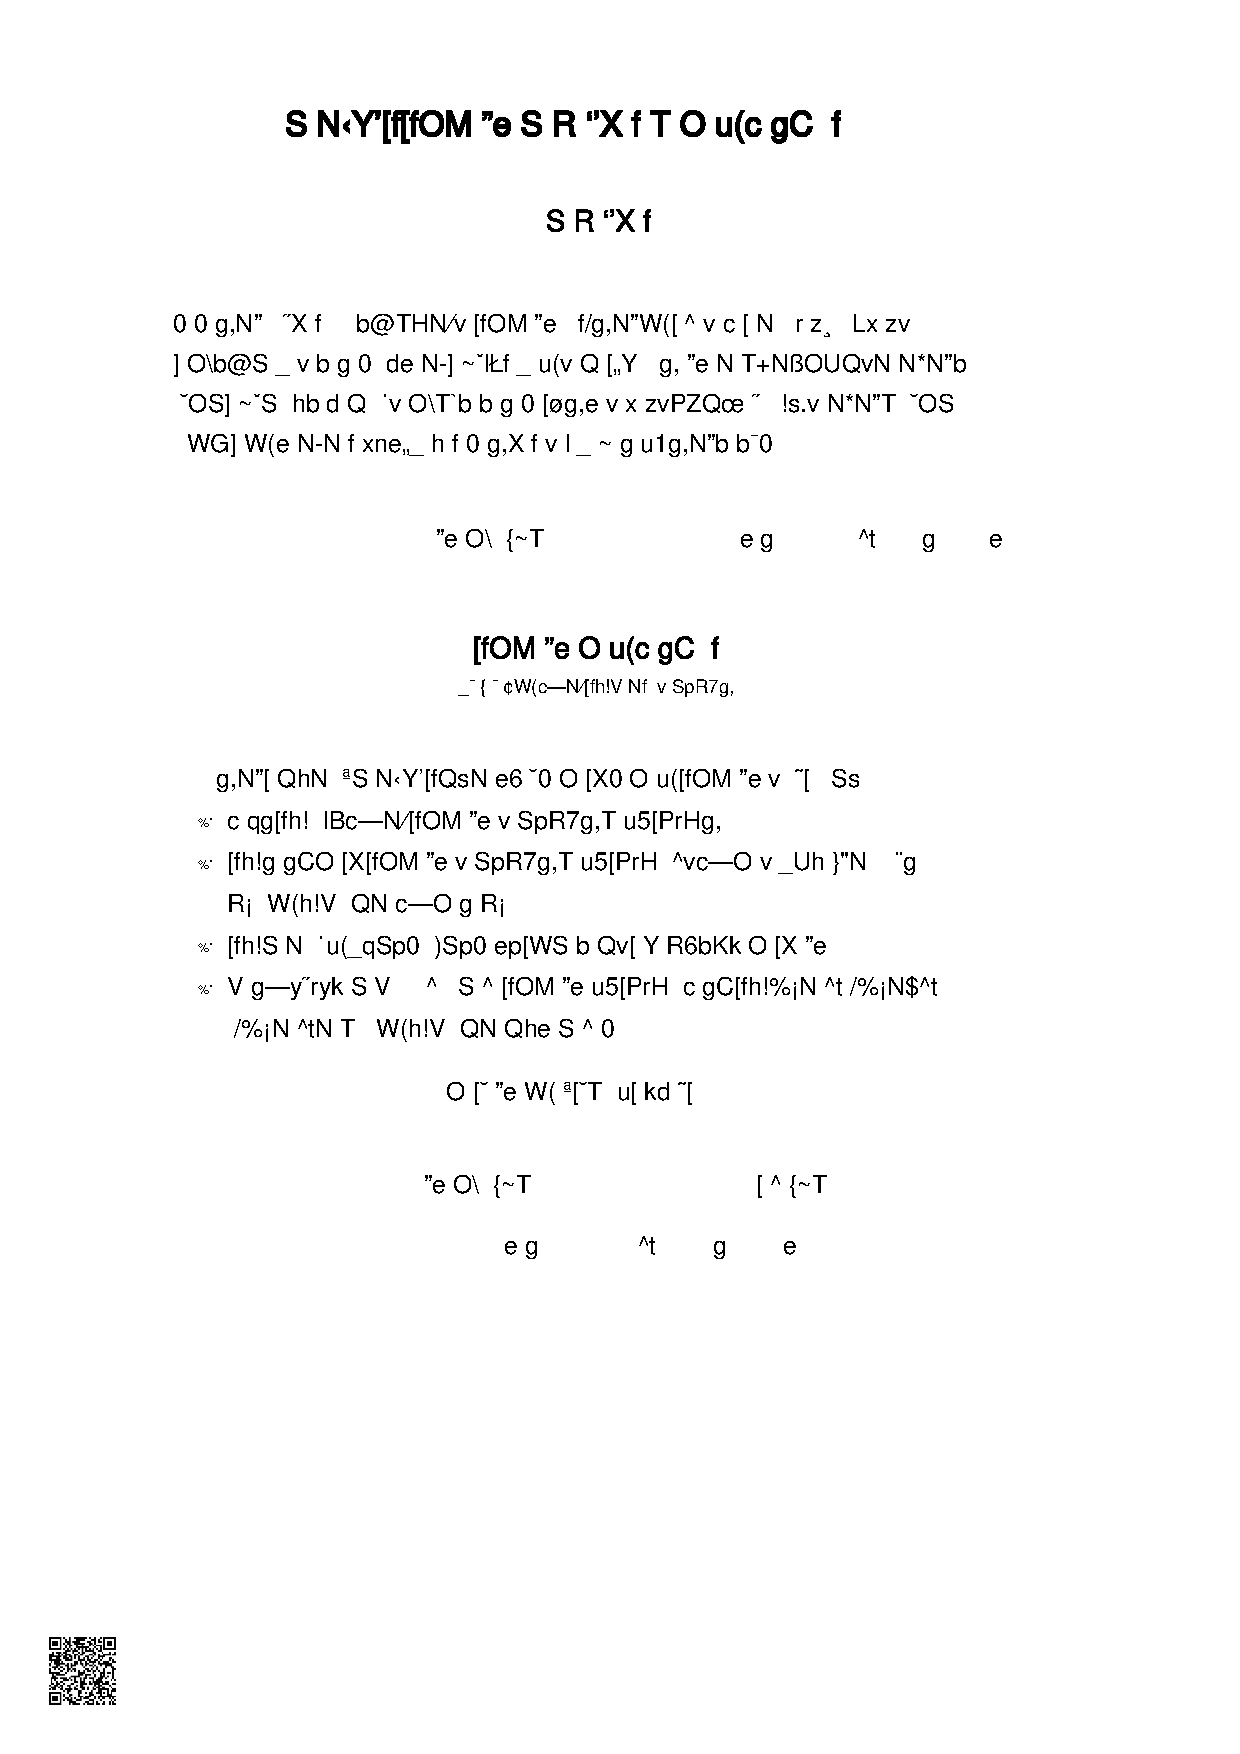
\includegraphics[height = 1.2448\textheight]{img/lwsm_180xxxxxxx.pdf}
		}
	\end{textblock}
}

% vim:ts=4:sw=4

\end{document}

% vim:ts=4:sw=4